\section{Studio dei Nuclei}
\subsection{Diffusione Elastica elettrone Nucleo}
Per superare i limiti dati dallo studio con le particelle Alfa, si cominciò a sfruttare gli elettroni.
Questi sono stati la sonda "principe" per lo studio del nucleo ma anche dei nucleoni (protoni e neutroni), perché:
\begin{itemize}
\item possono essere considerati puntiformi, infatti per quanto ne sappiamo non possiedono struttura, e quindi le loro dimensioni non impattano nello studio del nucleone.
\item interagiscono solo per interazione elettromagnetica, a differenza per dire delle particelle alfa che interagiscono anche tramite la forza forte rendendo difficoltosa la distinzione tra i due tipi di interazione.
\end{itemize}

Gli elettroni vengono usati dagli anni 50, ossia da quando è possibile costruire degli acceleratori.
L'innovazione in questo campo è stata data dall'energia a cui si riesce ad accelerare gli elettroni portando a nuove scoperte.

Perché è così importante ottenere energie sempre più elevate per avere maggiore risoluzione sulla struttura?
Il motivo si basa sulla relazione di de Briglie, quando noi vogliamo studiare la struttura, la lunghezza d'onda della sonda deve essere più piccola della struttura che andiamo a studiare.
\begin{equation}
\begin{split}
\lambda=\frac{h}{\varphi}\leq 2R\\
\frac{2\pi\hbar}{p}=2R\\
pc=\frac{2\pi\hbar}{2R}
\end{split}
\end{equation}
Quest'ultima formula si può scrivere grazie alla formula di Einstein per le energie, in quanto gli elettroni diventano relativistici ad energie di accelerazione molto basse.
\begin{equation}
\begin{split}
E^2 &=p^2c^2+m^2c^4\\
p^2c^2 \gg m^2c^4 &\hspace{0.5cm}\to\hspace{0.5cm}E=pc
\end{split}
\end{equation}
Si ottiene quindi che l'energia è pari a 
\begin{equation}
E=2\pi\frac{197MeV\cdot fm}{2R}
\end{equation}

Questa valutazione energetica rende il raggio del nucleo
\begin{equation}
r_{nucleo}=r_0A^{1/3}
\end{equation}
che, come già visto nel caso dell'oro corrisponde a $r_{Au}=1.2\sqrt[3]{197}=6,98 fm$.
Il che corrisponde ad un'energia di
\begin{equation}
pc=\frac{2\pi\cdot 197MeV\cdot fm}{2\cdot6,98}=89MeV
\end{equation}
Se quindi voglio usare gli elettroni per studiare questo tipo di nucleo dovrò accelerare gli elettroni ad un minimo di $89 MeV$.
Aumentando ulteriormente l'energia poi si avrà che diminuisce ancora la lunghezza d'onda portandomi alla risoluzione pure del nucleone;
ciò che cambia rispetto al nucleo è che non avrò più collisione elastica e quindi non avrò più il protone intatto dopo la collisione e di conseguenza cambierà anche la sezione d'urto.
L'energia necessaria per lo studio del protone ($r_{prot.}\sim 1fm$) è $E=pc=0,5GeV$.
Per lo studio del quark poi serviranno energie ancora maggiori, pari a 6,1 TeV.

\paragraph{Sezione d'urto di Mott}

Le assunzioni fatte per il calcolo della sezione d'urto di Rutherford sono state:
\begin{enumerate}
\item Interazione puramente coulombiana
\item Ne proiettile ne bersaglio possiedono spin
\end{enumerate}
Le assunzione su cui si baserà la sezione d'urto di Mott, necessaria alla descrizione dell'interazione nucleo elettrone, sono:
\begin{enumerate}
\item Bersaglio privo di spin
\item Proiettile con spin
\end{enumerate}
Tramite questo piccolo cambio si ottiene che la sezione d'urto di Mott diventa:
\begin{equation}
\left(\frac{d\sigma}{d\Omega}\right)_{Mott} *=\left(\frac{d\sigma}{d\Omega}\right)_{Ruth}\left(1-\beta^2\sin^2\frac{\theta}{2}\right)
\end{equation}
con $\beta=v/c$.
L'asterisco sta ad indicare che trascuriamo gli effetti di rinculo.
Si suppone quindi che il nucleo abbia massa infinita e che quindi l'elettrone abbia energia cinetica iniziale uguale a quella finale, questa assunzione è possibile fino al GeV perché al di sopra le energie iniziano a diventare confrontabili.
Il termine moltiplicativo della sezione d'urto di Rutherford sopra è ciò che indica lo spin dell'elettrone, studiamo quindi il suo significato.
\begin{equation}
\begin{split}
\beta&\to1\\
v&\to c\\
1-\beta^2\sin^2\frac{\theta}{2}&\to \cos^2\frac{\theta}{2}
\end{split}
\end{equation}
Questo comporta una grande modifica alla sezione d'urto di Rutherford, in quanto viene inibito il back scattering caratteristico dell'esperimento con il bersaglio d'oro, e ciò è dovuto allo spin dell'elettrone.
Il tutto si spiega grazie ad una quantità definita come elicità
\begin{equation}
h=\frac{\bar s\cdot \bar p}{|s||p|}
\end{equation}
Praticamente è la proiezione dello spin nella direzione della quantità di moto.
Lo spin è una proprietà caratteristica delle particelle che classicamente viene indicata come una rotazione della particella attorno a se stessa, molto utile a comprendere il concetto ma scorretto da un punto di vista reale (elettrone puntiforme non ha rotazione).
In questo tipo di interazione il momento angolare e l'elicità si conservano.
\begin{figure}[h]
\centering
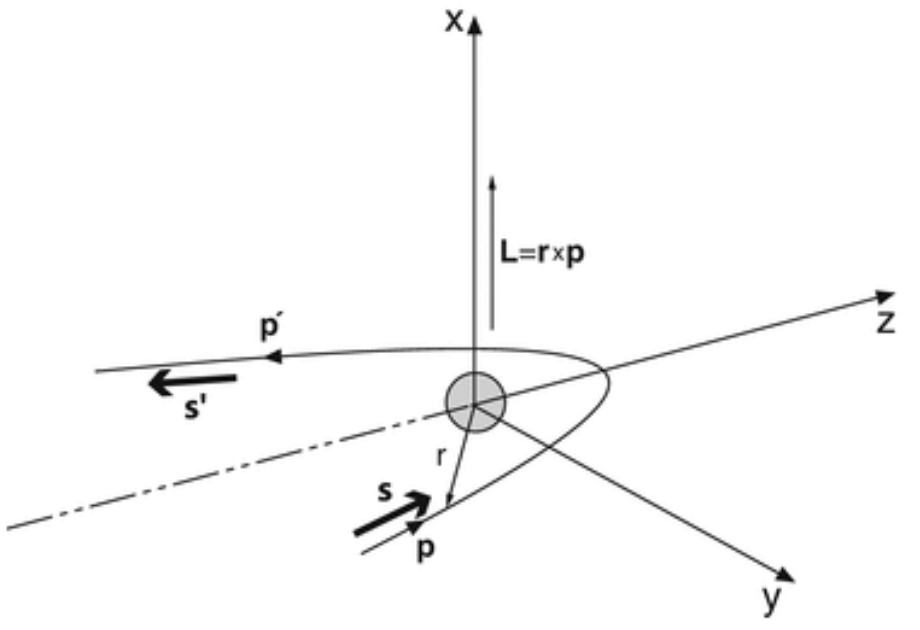
\includegraphics[width=150pt]{fig2_01}
\caption{Backscattering di elettrone}
\label{fig:2.01}
\end{figure}
Per la conservazione della quantità di moto un evento di backscattering richiede un'inversione dell'elicità, ma siccome anche l'elicità dell'elettrone si deve conservare si ottiene che il backscattering è inibito.

La conservazione dell'elicità dipende da regole naturali e riguarda le particelle con velocità prossime a quella della luce.
Nel caso infatti in cui la particella ha una velocità non relativistica ci si può osservare il modo da più punti superando la particella e questo genera un cambio di elicità.
Nel caso invece in cui la particella ha velocità $v\to c$ l'elicità è definita e viene denominata chiralità.
Ciò vuol dire che gli elettroni possiedono più componenti di elicità ma quando si avvicinano a velocità relativistiche ne rimane solamente una. Questa è una legge che deriva dall'esperienza, non ha quindi un motivo se non l'osservazione.
\'E oltre un'evidenza dell'equazione di Dirac e da osservazioni della forza debole.
Questo indica che la natura non è simmetrica e ci deve andare bene (la materia preferisce chiralità sinistra, l'antimateria la destra).

Si ha inoltre che per far cambiare l'elicità dell'elettrone bisognerebbe avere un'interazione magnetica, non basta quella elettrostatica, è necessario quindi che anche il bersaglio abbia spin. 

Questi sono i due motivi dietro la conservazione di parità.

\paragraph{Studio dell'interazione sonda bersaglio}
\begin{figure}[h]
\centering
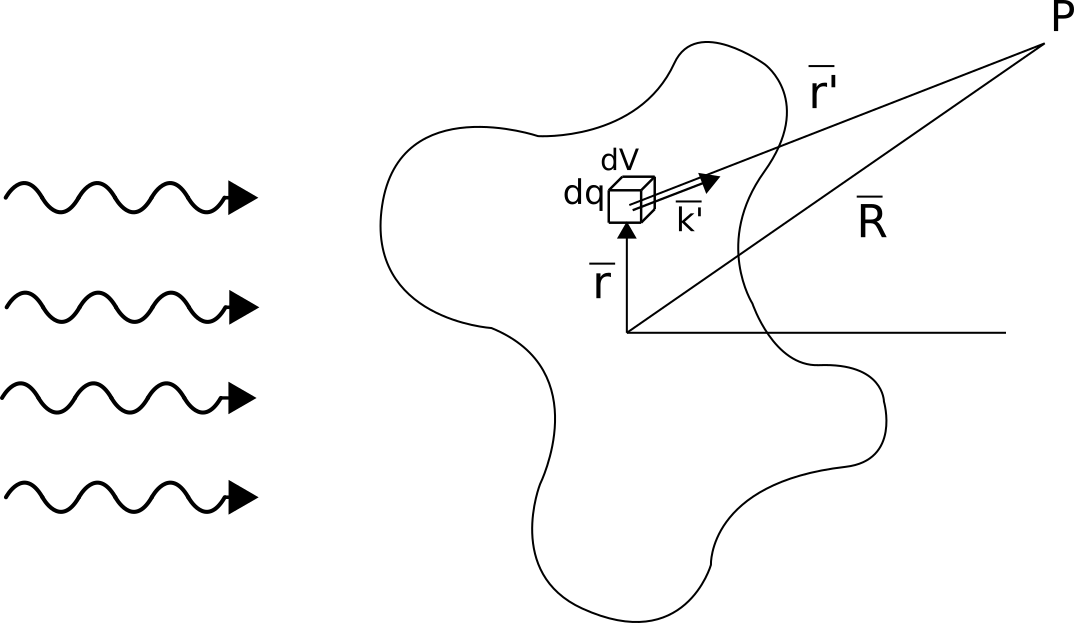
\includegraphics[width=200pt]{fig2_02}
\caption{Rappresentazione dell'interazione di un fascio con una distribuzione di carica}
\label{fig:2.02}
\end{figure}
Supponiamo di avere un fascio di elettroni incidenti su un bersaglio esteso.
Data una distribuzione qualsiasi di carica colpita da un fascio di elettroni rappresentato come un'onda piana $e^{ikr}$, si può prendere un sistema di coordinate centrato al centro della carica.
L'interazione che si ottiene può essere vista come la somma di tutte le interazioni derivate dai punti della carica. 
Per visualizzare questo si consideri un cubetto di carica $dq$ e volume $dV$, con coordinata $\bar r$ rispetto al centro di coordinate. 
Analogamente a come si fa in ottica, supponiamo che dopo l'interazione si generi da quel punto un'onda sferica.
A questo punto si analizza l'onda ottenuta nel punto P, virtualmente all'infinito, di coordinata $\bar{R}$ rispetto al centro del nucleo e con distanza $\bar{r'}$ rispetto al volumetto infinitesimo di carica.
Si può ora sommare il contributo di ogni carica infinitesima per ottenere il contributo totale nel punto P dato da tutto il nucleo.
Prendendo come onda piana incidente un'onda di energia:
\begin{equation}
E=E_0\cdot e^{ikr}
\end{equation}
il contributo infinitesimo dell'onda generata è rappresentato da
\begin{equation}
A=E_0 e^{ikr}\frac{a}{r'}e^{ik'r'}=\frac{aE_0}{r'}e^{i(kr+k'r')}
\end{equation}
dove $a$ è l'ampiezza di diffusione, ovvero la sezione d'urto elementare di Mott.
\begin{equation}
\begin{split}
\bar{r}+\bar{r'}&=\bar{R}\\
\bar{k}\bar{r}&=\bar{k'}\bar{R}-\bar{k'}\bar{r'}\\
\end{split}
\end{equation}

\begin{equation}
\begin{split}
R\to\infty &\hspace{0.5cm}r'\approx R\hspace{0.5cm}k'||R\\
M_{nucleo}\to\infty &\hspace{0.5cm}|k'|=|k|=k
\end{split}
\end{equation}
Prese le approssimazioni qui sopra descritte si ottiene
\begin{equation}
A=\frac{aE_0}{R}e^{ikR}\cdot e^{i(k-k')r}
\end{equation}
Integrando poi su tutto il volume
\begin{equation}
\int A=\frac{aE_0}{RQ}\int \rho_e(r)e^{-i\Delta kr)}
\end{equation}
Dove $Q$ è la carica totale e $\rho$ è la densità di carica.
Sappiamo dalla sezione precedente che la quantità di moto trasferita si definisce come
\begin{equation}
\bar{q}=\hbar \bar{\Delta K}
\end{equation}
Sostituendo si ottiene
\begin{equation}
=\frac{aE_0}{RZe}\int \rho_e(r)e^{-i\frac{q}{\hbar}r}
\end{equation}
Essendo $a$ la sezione d'urto di Mott ve ne si può evidenziare la dipendenza cinematica dovuta alla sua dipendenza dalla sezione d'urto di Rutherford ($\propto 1/q^4$). 
Non sarà dimostrato ma bisogna sapere che $d\sigma/d\Omega$ dipende da $|A|^2$.
Si può finalmente trovare la sezione d'urto
\begin{equation}
\begin{split}
\left(\frac{d\sigma}{d|Omega}\right)_\theta &=\left(\frac{d\sigma}{d|Omega}\right)_{Mott}\biggl| \int\rho_e(r)\cdot e^{-i\frac{q}{\hbar}}dr\biggl|^2\\
&=\left(\frac{d\sigma}{d\Omega}\right)_{Mott}|F(\rho,q)|^2
\end{split}
\end{equation}
L'ultimo fattore della formula sopra si chiama fattore di forma nucleare e coincide con la trasformata di Fourier della distribuzione di carica nel nucleo.
\begin{equation}
F(\rho, q)=\int \rho_e(r)e^{-i\frac{q}{\hbar}r}dr
\end{equation}
In pratica quando un fascio di elettroni interagisce con una densità di carica di ottiene o stesso effetto che si ha con un'onda piana che fa diffrazione da una fenditura.

\paragraph{Esempi}
\begin{figure}[h]
\centering
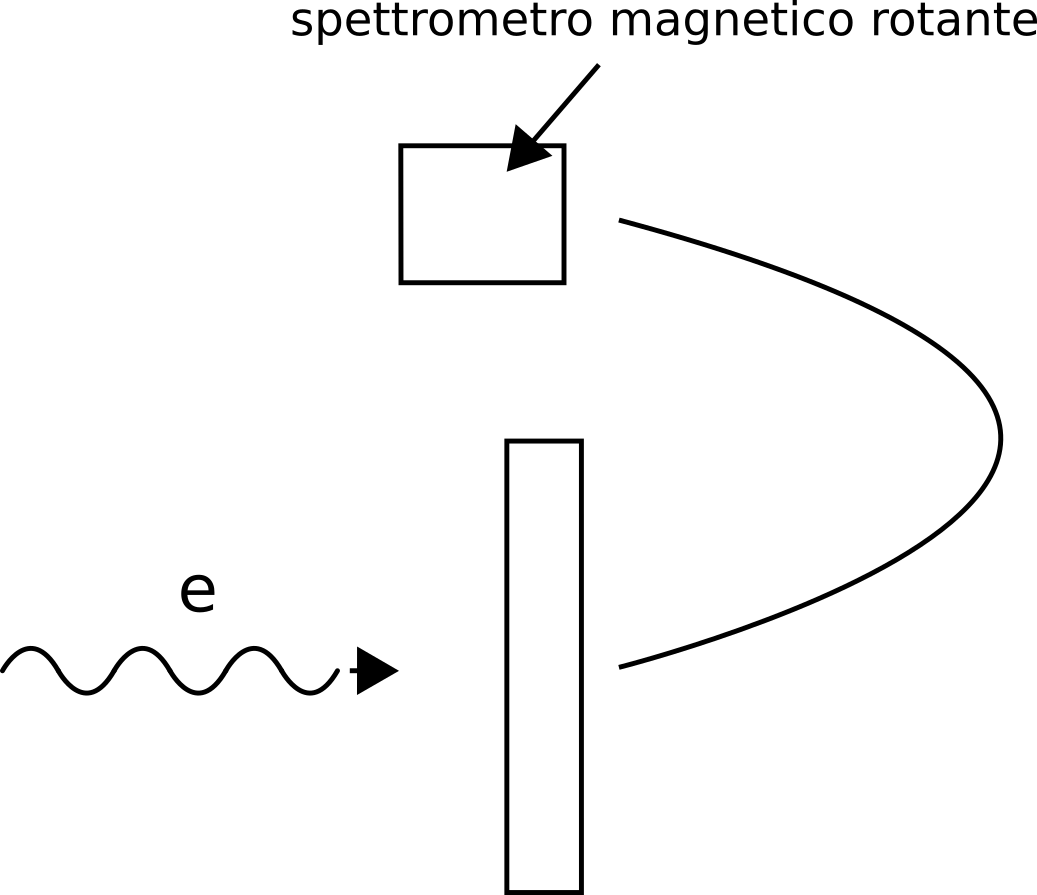
\includegraphics[width=150pt]{fig2_03}
\end{figure}
In figura è mostrato un esperimento di scattering dove c'è un fascio interagente con un bersaglio rivelato da uno spettrometro magnetico rotante che poteva misurare l'energia delle particelle a più angoli di diffusione. Il grafico ottenuto da un'esperienza di questo tipo era del tipo mostrato nel grafico sotto.
\begin{figure}[h]
\centering
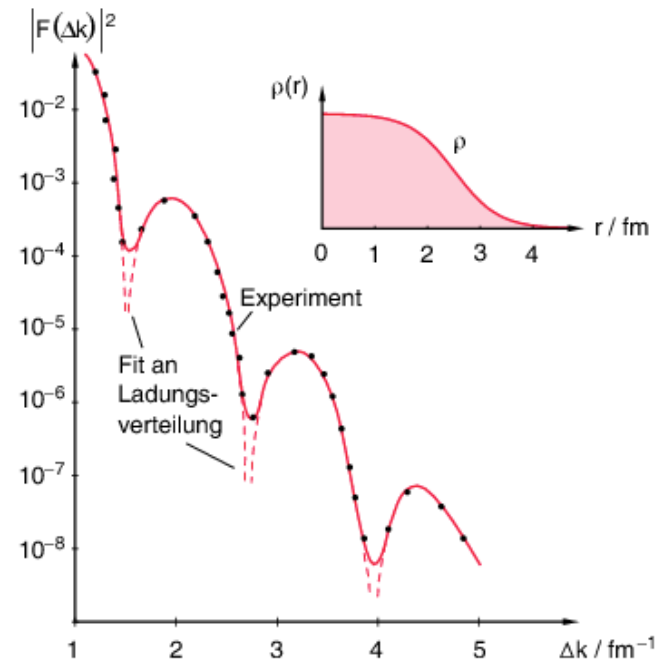
\includegraphics[width=180pt]{fig2_04}
\end{figure}
Come si può notare dal grafico la distribuzione di carica era in un certo modo inaspettata ma rispecchia i ragionamenti fatti riguardo la variabilità della sezione di Mott in base alla distribuzione.
La distribuzione di Mott infatti viene modulata come la trasformata di Fourier della distribuzione di carica e se, per esempio, la distribuzione di carica fosse puntiforme sarebbe uguale alla delta di Dirac, non avendo nessuna deviazione dalla sezione di Mott prevista, in quanto la trasformata di una delta è una distribuzione uniforme. 
Dai dati sperimentali si ottenne però il grafico sopra, dovuto al fatto di non poter considerare il nucleo come puntiforme.
Come si può notare, i dati sperimentali evidenziano un importante parallelismo con l'effetto di diffrazione della luce su una fenditura.

Questo rende possibile la determinazione del raggio del nucleo sfruttando le stesse formule usate per trovare la dimensione di una fenditura.
Si prenda per esempio un nucleo di Stagno $^{124}Sn$ e vi si faccia collimare un fascio di elettroni con energia $E=330MeV$;
il raggio del nucleo sarà
\begin{equation}
r=0,61 \frac{\lambda}{\sin\theta}
\end{equation} 
La lambda corrisponde a $\lambda=hc/E=3,7fm$ e il primo minimo si trova a $\theta=45^o$, si ottiene quindi un raggio pari a $r=3,19fm$.

Questi esperimenti ci hanno permesso di determinare la distribuzione di carica del nucleo, che corrisponde all'incirca alla distribuzione di massa.
Ciò che si è notato è che il nucleo non è propriamente una sfera rigida ma ha un andamento come quello mostrato in figura sotto.
\begin{figure}[h]
\centering
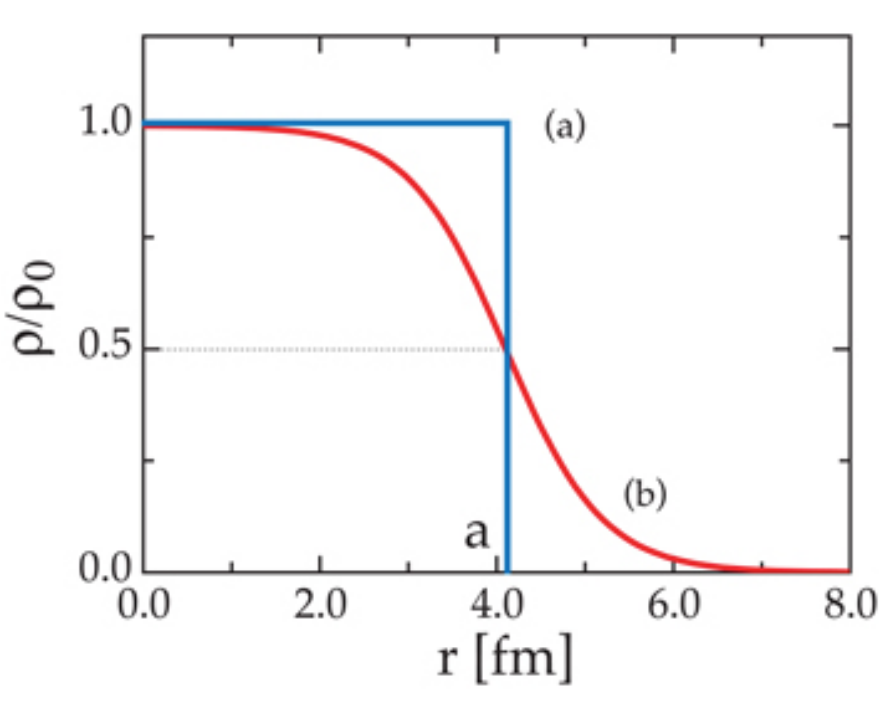
\includegraphics[width=150pt]{fig2_05}
\end{figure}

Questa corrisponde alla distribuzione di Saxon-Woods data dalla formula
\begin{equation}
\rho(r)=\frac{\rho_0}{1+exp\left(\frac{r-a}{b}\right)}
\end{equation}
dove $a=118A^{1/3}=0,48fm$ e $b=0,55\pm 0,07fm$.
Questo mostra la presenza di una zona dove la densità del nucleo diminuisce gradualmente.

Qual è la densità di materia nel nucleo?
\begin{equation}
\begin{split}
R&=R_0A^{1/3}\\
\rho_{M}&=\frac{M}{V}=\frac{A\cdot u}{\frac{4}{3}\pi R^3}\\
&=\frac{A\cdot u}{\frac{4}{3}\pi R_0^3A}\approx10^{17}\frac{kg}{m^3}
\end{split}
\end{equation}
dove $A$ corrisponde al numero di massa del nucleo e $u$ è l'unità di massa atomica. 
Dalla divisione di A per A si nota come la densità non dipende dal tipo di nucleo ma è uguale per tutti i nuclei.